% Sections for Phases 3-6; filled in when their records exist.
\subsection{Tuned hyper-parameters}\label{sec:hpo}
Every method received 20 random-search trials per dataset (\S\ref{sec:protocol}). The winner of
each method and dataset was chosen on the seed-0 validation AUROC only and then re-run on
seeds 0--4. Tables~\ref{tab:hpo} and~\ref{tab:hpopairs} repeat the main-stage analysis on these
\HpoRecords{} runs.

\begin{table}[t]
  \centering
  \caption{Test AUROC (mean{\tiny$\pm$sd} over \HpoSeeds{} seeds) with tuned hyper-parameters.
  Layout as in Table~\ref{tab:main}.}
  \label{tab:hpo}
  \small
  \resizebox{\textwidth}{!}{\begin{tabular}{lcccccc}
\toprule
Dataset & LR & DT & RF & GBDT & TabResNet & IMN \\
\midrule
kr-vs-kp & 0.994{\tiny$\pm$0.002} & 0.995{\tiny$\pm$0.002} & 0.995{\tiny$\pm$0.002} & \textbf{0.999{\tiny$\pm$0.000}} & 0.999{\tiny$\pm$0.001} & 0.999{\tiny$\pm$0.001} \\
credit-g & 0.788{\tiny$\pm$0.052} & 0.716{\tiny$\pm$0.052} & 0.794{\tiny$\pm$0.052} & 0.789{\tiny$\pm$0.057} & \textbf{0.796{\tiny$\pm$0.048}} & 0.791{\tiny$\pm$0.045} \\
vehicle & 0.944{\tiny$\pm$0.009} & 0.854{\tiny$\pm$0.018} & 0.925{\tiny$\pm$0.005} & 0.924{\tiny$\pm$0.011} & \textbf{0.958{\tiny$\pm$0.007}} & 0.953{\tiny$\pm$0.011} \\
kc1 & 0.811{\tiny$\pm$0.013} & 0.749{\tiny$\pm$0.037} & \textbf{0.835{\tiny$\pm$0.007}} & 0.820{\tiny$\pm$0.008} & 0.814{\tiny$\pm$0.012} & 0.813{\tiny$\pm$0.010} \\
blood-transfusion & \textbf{0.737{\tiny$\pm$0.032}} & 0.688{\tiny$\pm$0.048} & 0.699{\tiny$\pm$0.037} & 0.694{\tiny$\pm$0.038} & 0.722{\tiny$\pm$0.054} & 0.669{\tiny$\pm$0.058} \\
phoneme & 0.810{\tiny$\pm$0.009} & 0.869{\tiny$\pm$0.011} & 0.919{\tiny$\pm$0.007} & \textbf{0.954{\tiny$\pm$0.005}} & 0.936{\tiny$\pm$0.005} & 0.944{\tiny$\pm$0.005} \\
adult & 0.902{\tiny$\pm$0.003} & 0.900{\tiny$\pm$0.003} & 0.910{\tiny$\pm$0.003} & \textbf{0.928{\tiny$\pm$0.001}} & 0.914{\tiny$\pm$0.002} & 0.912{\tiny$\pm$0.002} \\
Australian & 0.921{\tiny$\pm$0.003} & 0.921{\tiny$\pm$0.016} & 0.937{\tiny$\pm$0.012} & \textbf{0.943{\tiny$\pm$0.016}} & 0.927{\tiny$\pm$0.020} & 0.920{\tiny$\pm$0.023} \\
segment & 0.995{\tiny$\pm$0.001} & 0.989{\tiny$\pm$0.003} & 0.998{\tiny$\pm$0.001} & \textbf{0.999{\tiny$\pm$0.000}} & 0.998{\tiny$\pm$0.000} & 0.997{\tiny$\pm$0.001} \\
jungle\_chess & 0.803{\tiny$\pm$0.003} & 0.856{\tiny$\pm$0.005} & 0.896{\tiny$\pm$0.003} & 0.977{\tiny$\pm$0.001} & \textbf{0.981{\tiny$\pm$0.001}} & 0.980{\tiny$\pm$0.001} \\
jasmine & 0.854{\tiny$\pm$0.008} & 0.838{\tiny$\pm$0.007} & \textbf{0.871{\tiny$\pm$0.005}} & 0.866{\tiny$\pm$0.009} & 0.865{\tiny$\pm$0.009} & 0.861{\tiny$\pm$0.012} \\
sylvine & 0.966{\tiny$\pm$0.003} & 0.957{\tiny$\pm$0.009} & 0.975{\tiny$\pm$0.001} & \textbf{0.985{\tiny$\pm$0.002}} & 0.980{\tiny$\pm$0.003} & 0.977{\tiny$\pm$0.002} \\
\bottomrule
\end{tabular}
}\\[4pt]
  \resizebox{\textwidth}{!}{\begin{tabular}{lcccccccc}
\toprule
Dataset & IMN & TM & Clause-LR & IMN-TM & IMN-TM (rand.) & IMN-Hybrid & TM-Gated & Paper IMN \\
\midrule
kr-vs-kp & 0.999{\tiny$\pm$0.001} & 0.997{\tiny$\pm$0.002} & 0.999{\tiny$\pm$0.001} & \textbf{0.999{\tiny$\pm$0.001}} & \textbf{0.999{\tiny$\pm$0.001}} & 0.999{\tiny$\pm$0.001} & 0.998{\tiny$\pm$0.001} & 0.999 \\
credit-g & 0.791{\tiny$\pm$0.045} & 0.792{\tiny$\pm$0.051} & 0.793{\tiny$\pm$0.051} & 0.799{\tiny$\pm$0.049} & 0.792{\tiny$\pm$0.061} & \textbf{0.799{\tiny$\pm$0.049}} & 0.766{\tiny$\pm$0.030} & 0.751 \\
vehicle & \textbf{0.953{\tiny$\pm$0.011}} & 0.922{\tiny$\pm$0.009} & 0.927{\tiny$\pm$0.008} & 0.936{\tiny$\pm$0.011} & 0.937{\tiny$\pm$0.005} & 0.937{\tiny$\pm$0.011} & 0.931{\tiny$\pm$0.010} & 0.957 \\
kc1 & 0.813{\tiny$\pm$0.010} & 0.804{\tiny$\pm$0.013} & 0.816{\tiny$\pm$0.007} & 0.816{\tiny$\pm$0.008} & 0.817{\tiny$\pm$0.010} & \textbf{0.818{\tiny$\pm$0.009}} & 0.815{\tiny$\pm$0.015} & 0.805 \\
blood-transfusion & 0.669{\tiny$\pm$0.058} & 0.698{\tiny$\pm$0.059} & 0.705{\tiny$\pm$0.065} & 0.706{\tiny$\pm$0.065} & \textbf{0.725{\tiny$\pm$0.057}} & 0.708{\tiny$\pm$0.066} & 0.715{\tiny$\pm$0.051} & 0.742 \\
phoneme & 0.944{\tiny$\pm$0.005} & 0.937{\tiny$\pm$0.005} & 0.943{\tiny$\pm$0.004} & 0.948{\tiny$\pm$0.004} & 0.945{\tiny$\pm$0.004} & \textbf{0.948{\tiny$\pm$0.004}} & 0.945{\tiny$\pm$0.004} & 0.950 \\
adult & 0.912{\tiny$\pm$0.002} & 0.905{\tiny$\pm$0.003} & 0.910{\tiny$\pm$0.003} & 0.912{\tiny$\pm$0.002} & 0.910{\tiny$\pm$0.002} & 0.912{\tiny$\pm$0.002} & \textbf{0.913{\tiny$\pm$0.002}} & 0.915 \\
Australian & 0.920{\tiny$\pm$0.023} & 0.924{\tiny$\pm$0.012} & 0.938{\tiny$\pm$0.010} & \textbf{0.939{\tiny$\pm$0.006}} & 0.938{\tiny$\pm$0.013} & 0.939{\tiny$\pm$0.005} & 0.936{\tiny$\pm$0.011} & 0.908 \\
segment & 0.997{\tiny$\pm$0.001} & 0.998{\tiny$\pm$0.001} & \textbf{0.999{\tiny$\pm$0.000}} & 0.998{\tiny$\pm$0.000} & 0.997{\tiny$\pm$0.001} & 0.996{\tiny$\pm$0.002} & 0.998{\tiny$\pm$0.002} & 0.994 \\
jungle\_chess & \textbf{0.980{\tiny$\pm$0.001}} & 0.969{\tiny$\pm$0.001} & 0.974{\tiny$\pm$0.001} & 0.975{\tiny$\pm$0.002} & 0.970{\tiny$\pm$0.001} & 0.975{\tiny$\pm$0.002} & 0.974{\tiny$\pm$0.002} & 0.978 \\
jasmine & 0.861{\tiny$\pm$0.012} & 0.856{\tiny$\pm$0.012} & 0.863{\tiny$\pm$0.008} & \textbf{0.876{\tiny$\pm$0.009}} & 0.869{\tiny$\pm$0.013} & 0.876{\tiny$\pm$0.009} & 0.862{\tiny$\pm$0.009} & 0.865 \\
sylvine & 0.977{\tiny$\pm$0.002} & 0.971{\tiny$\pm$0.005} & 0.976{\tiny$\pm$0.003} & 0.981{\tiny$\pm$0.002} & 0.978{\tiny$\pm$0.003} & \textbf{0.981{\tiny$\pm$0.002}} & 0.979{\tiny$\pm$0.002} & 0.981 \\
\bottomrule
\end{tabular}
}
\end{table}
\begin{table}[t]
  \centering\small
  \caption{Preregistered comparisons, tuned hyper-parameters (\HpoDatasets{} datasets).
  $^\ast$: Holm-corrected $p<0.05$.}
  \label{tab:hpopairs}
  \begin{tabular}{llrcccc}
\toprule
Q & Comparison $A$ vs.\ $B$ & mean $A{-}B$ & 95\% bootstrap CI & W/L & $p$ & $p_\text{Holm}$ \\
\midrule
Q1 & IMN-TM vs.\ TM & +0.0094 & [+0.0065, +0.0125] & 12/0 & \ensuremath{4.9\times 10^{-4}} & 0.005$^\ast$ \\
Q2 & IMN-TM vs.\ IMN & +0.0058 & [-0.0010, +0.0136] & 9/3 & 0.129 & 0.776 \\
Q3 & IMN-Hybrid vs.\ IMN & +0.0059 & [-0.0010, +0.0139] & 8/4 & 0.176 & 0.776 \\
Q3 & IMN-Hybrid vs.\ IMN-TM & +0.0001 & [-0.0004, +0.0006] & 7/5 & 0.380 & 0.904 \\
Q4 & TM-Gated vs.\ LR & +0.0254 & [-0.0031, +0.0629] & 9/3 & 0.301 & 0.904 \\
Q4 & TM-Gated vs.\ TM & +0.0049 & [-0.0016, +0.0096] & 11/1 & 0.034 & 0.239 \\
Q4 & TM-Gated vs.\ IMN & +0.0013 & [-0.0075, +0.0116] & 8/4 & 0.519 & 0.904 \\
Q5 & IMN-TM vs.\ Clause-LR & +0.0036 & [+0.0015, +0.0060] & 10/2 & 0.003 & 0.031$^\ast$ \\
Q6 & IMN-TM vs.\ IMN-TM (rand.) & +0.0007 & [-0.0035, +0.0037] & 8/4 & 0.151 & 0.776 \\
R & IMN vs.\ TabResNet & -0.0061 & [-0.0155, -0.0001] & 1/11 & 0.027 & 0.215 \\
\bottomrule
\end{tabular}

\end{table}
\begin{figure}[t]
  \centering
  \begin{subfigure}[t]{0.49\textwidth}\centering
    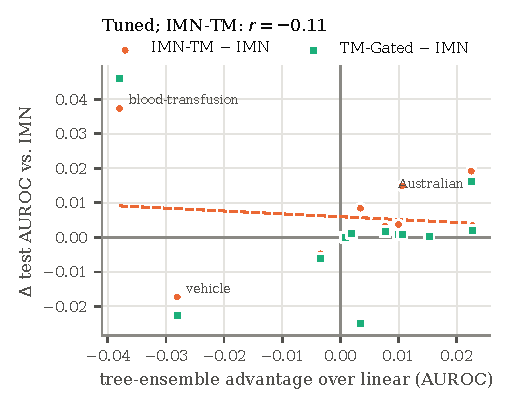
\includegraphics[width=\linewidth]{figures/hpo_final_gap.pdf}
    \caption{Gain over \imn{} vs.\ the tree-ensemble advantage, tuned.}
    \label{fig:hpogap}
  \end{subfigure}\hfill
  \begin{subfigure}[t]{0.49\textwidth}\centering
    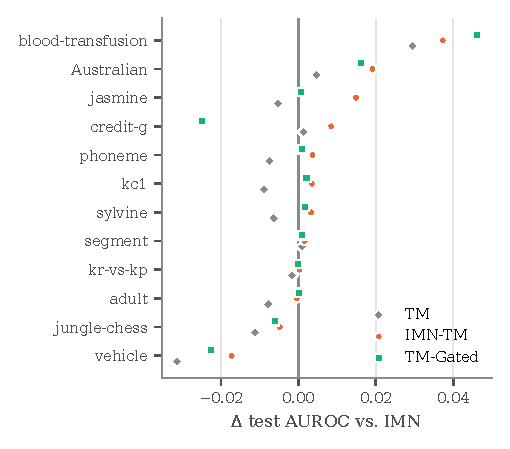
\includegraphics[width=\linewidth]{figures/hpo_final_delta.pdf}
    \caption{Per-dataset $\Delta$AUROC vs.\ \imn{}, tuned.}
    \label{fig:hpodelta}
  \end{subfigure}
  \caption{\textbf{Where the TM helps, after tuning.} Compare with Figure~\ref{fig:where}.}
  \label{fig:hpowhere}
\end{figure}

\paragraph{Tuning helps the clause models most.} \arm{IMN-TM} improves on its default
configuration on \TuneimntmWins{} of 12 datasets (\TuneimntmMean{} mean AUROC, to
\TuneimntmAuroc). \imn{} gains \TuneimnMean{} on \TuneimnWins{} datasets and TabResNet gains
\TunetabresnetMean. Random forests lose \TunerfMean, which shows that selecting on one
validation split is noisy. After tuning, \arm{IMN-TM} shares the best average rank with GBDT
(both \HpoRankimntm; \arm{IMN-Hybrid} \HpoRankimnhybrid, TabResNet \HpoRanktabresnet, \imn{}
\HpoRankimn; Figure~\ref{fig:ranks}). The critical difference is \HpoCD, however, so the leading
group cannot be separated statistically.

\paragraph{Preregistered questions.}
\begin{itemize}
  \item \textbf{Q1} is stronger than with defaults: \arm{IMN-TM} beats its source TM on
        \HpoimntmtmWins/12 datasets (\HpoimntmtmMean, Holm $p=\HpoimntmtmHolm$).
  \item \textbf{Q5} becomes significant. The per-example generator beats a single global re-fit
        of the same clause weights by \HpoimntmclauselrMean{}
        (\HpoimntmclauselrWins/\HpoimntmclauselrLosses, Holm $p=\HpoimntmclauselrHolm$).
  \item \textbf{Q2} moves in favour of \arm{IMN-TM} (\HpoimntmimnMean,
        \HpoimntmimnWins/\HpoimntmimnLosses) but remains unresolved: the confidence interval
        includes zero. One dataset dominates the mean: on \HpoImntmImnBest{} the tuned \imn{}
        lost \TuneimnWorst{} against its own default, a selection failure on a dataset of
        748 rows. Without it the mean difference is \HpoImntmImnMeanNoBest.
  \item \textbf{Q6} is unchanged. Random clauses remain as accurate as learned ones
        (\HpoimntmimntmrandMean).
  \item \textbf{R}: tuned \imn{} falls behind tuned TabResNet (\HpoimntabresnetMean,
        \HpoimntabresnetWins/\HpoimntabresnetLosses, Holm $p=\HpoimntabresnetHolm$). The paper
        reports them level.
\end{itemize}

\paragraph{The default-HP pattern does not survive tuning.} With tuning, \imn{} gains most on
exactly the datasets where clauses had helped: \TuneimnBest. The correlation between the
\arm{IMN-TM} gain and the tree-ensemble advantage falls from $r=\MainGapCorr$ to
$r=\HpoGapCorr$ (Figure~\ref{fig:hpowhere}). The default-HP result should therefore be read as
follows. The clause basis gives the hypernetwork a good inductive bias for threshold-shaped
problems without any search. A tuned hyperplane model closes most of that gap, at a much higher
search cost.

\paragraph{Explanations after tuning.} Local fidelity is unchanged (\arm{IMN-TM}
\HpoFidimntm{} vs.\ \imn{} \HpoFidimn) and self-consistency stays high (\HpoSelfimntm). The tuned
clause models choose weaker L1 penalties, though, and their explanations grow from
\MainClausesimntm{} to \HpoClausesimntm{} rules for 90\% of the evidence. An accuracy-only
search therefore trades away explanation length; a search that also scores explanation size
would need an explicit constraint.
\subsection{Tier 2: twenty larger datasets}\label{sec:tier2}
Tier~2 covers the remaining AutoML-benchmark datasets. They have up to 324k training rows,
up to 4{,}296 features and up to 100 classes. Three are excluded (D25): guillermo and robert
fail OpenML's checksum, and albert cannot be downloaded. The remaining \TiertwoDatasets{}
datasets are run with \TiertwoSeeds{} seeds and default hyper-parameters (\TiertwoRecords{}
runs). All runs completed; \TiertwoSkipped{} were skipped for size.

Two preregistered caps keep the cost bounded (D24):
\begin{itemize}
  \item neural training stops after 50{,}000 steps;
  \item the source TM trains for at most 20 epochs.
\end{itemize}
The step cap binds on \TiertwoCappedN{} of the \TiertwoDatasets{} datasets.
Tables~\ref{tab:t2} and~\ref{tab:t2pairs} report the results.

\begin{table}[t]
  \centering
  \caption{Tier 2: test AUROC (mean{\tiny$\pm$sd} over \TiertwoSeeds{} seeds), default
  hyper-parameters with the step cap. Layout as in Table~\ref{tab:main}.}
  \label{tab:t2}
  \small
  \resizebox{\textwidth}{!}{\begin{tabular}{lcccccc}
\toprule
Dataset & LR & DT & RF & GBDT & TabResNet & IMN \\
\midrule
mfeat-factors & 0.997{\tiny$\pm$0.001} & 0.931{\tiny$\pm$0.017} & 0.998{\tiny$\pm$0.001} & 0.998{\tiny$\pm$0.000} & \textbf{0.999{\tiny$\pm$0.000}} & 0.998{\tiny$\pm$0.000} \\
KDDCup09\_appetency & 0.770{\tiny$\pm$0.009} & 0.527{\tiny$\pm$0.011} & 0.791{\tiny$\pm$0.006} & \textbf{0.807{\tiny$\pm$0.003}} & 0.744{\tiny$\pm$0.011} & 0.759{\tiny$\pm$0.003} \\
airlines & 0.680{\tiny$\pm$0.002} & 0.589{\tiny$\pm$0.001} & 0.693{\tiny$\pm$0.003} & \textbf{0.704{\tiny$\pm$0.002}} & 0.677{\tiny$\pm$0.003} & 0.676{\tiny$\pm$0.004} \\
bank-marketing & 0.904{\tiny$\pm$0.003} & 0.702{\tiny$\pm$0.003} & 0.928{\tiny$\pm$0.004} & \textbf{0.930{\tiny$\pm$0.001}} & 0.904{\tiny$\pm$0.002} & 0.903{\tiny$\pm$0.002} \\
cnae-9 & \textbf{0.995{\tiny$\pm$0.003}} & 0.911{\tiny$\pm$0.004} & 0.993{\tiny$\pm$0.002} & 0.970{\tiny$\pm$0.006} & 0.992{\tiny$\pm$0.004} & 0.983{\tiny$\pm$0.004} \\
nomao & 0.986{\tiny$\pm$0.001} & 0.928{\tiny$\pm$0.004} & 0.993{\tiny$\pm$0.001} & \textbf{0.993{\tiny$\pm$0.001}} & 0.986{\tiny$\pm$0.000} & 0.983{\tiny$\pm$0.001} \\
Amazon\_employee\_access & 0.845{\tiny$\pm$0.012} & 0.645{\tiny$\pm$0.023} & 0.849{\tiny$\pm$0.020} & \textbf{0.857{\tiny$\pm$0.018}} & 0.848{\tiny$\pm$0.010} & 0.847{\tiny$\pm$0.010} \\
higgs & 0.684{\tiny$\pm$0.002} & 0.624{\tiny$\pm$0.001} & 0.799{\tiny$\pm$0.005} & \textbf{0.801{\tiny$\pm$0.004}} & 0.721{\tiny$\pm$0.006} & 0.705{\tiny$\pm$0.004} \\
numerai28.6 & \textbf{0.529{\tiny$\pm$0.002}} & 0.503{\tiny$\pm$0.003} & 0.516{\tiny$\pm$0.006} & 0.523{\tiny$\pm$0.001} & 0.502{\tiny$\pm$0.009} & 0.521{\tiny$\pm$0.007} \\
shuttle & 0.961{\tiny$\pm$0.005} & 0.956{\tiny$\pm$0.043} & \textbf{1.000{\tiny$\pm$0.000}} & 0.578{\tiny$\pm$0.028} & 0.947{\tiny$\pm$0.030} & 0.906{\tiny$\pm$0.031} \\
Fashion-MNIST & 0.981{\tiny$\pm$0.000} & 0.883{\tiny$\pm$0.002} & 0.991{\tiny$\pm$0.000} & \textbf{0.993{\tiny$\pm$0.000}} & 0.985{\tiny$\pm$0.001} & 0.984{\tiny$\pm$0.000} \\
APSFailure & 0.961{\tiny$\pm$0.002} & 0.853{\tiny$\pm$0.007} & 0.991{\tiny$\pm$0.002} & \textbf{0.992{\tiny$\pm$0.002}} & 0.987{\tiny$\pm$0.001} & 0.980{\tiny$\pm$0.006} \\
christine & 0.718{\tiny$\pm$0.009} & 0.636{\tiny$\pm$0.011} & 0.798{\tiny$\pm$0.018} & \textbf{0.811{\tiny$\pm$0.011}} & 0.737{\tiny$\pm$0.008} & 0.767{\tiny$\pm$0.007} \\
MiniBooNE & 0.937{\tiny$\pm$0.001} & 0.866{\tiny$\pm$0.003} & 0.980{\tiny$\pm$0.001} & \textbf{0.983{\tiny$\pm$0.001}} & 0.925{\tiny$\pm$0.006} & 0.907{\tiny$\pm$0.002} \\
riccardo & 0.995{\tiny$\pm$0.002} & 0.837{\tiny$\pm$0.009} & 0.998{\tiny$\pm$0.000} & \textbf{1.000{\tiny$\pm$0.000}} & 0.998{\tiny$\pm$0.001} & 0.998{\tiny$\pm$0.001} \\
dilbert & 0.994{\tiny$\pm$0.000} & 0.868{\tiny$\pm$0.004} & 0.998{\tiny$\pm$0.000} & \textbf{1.000{\tiny$\pm$0.000}} & 0.996{\tiny$\pm$0.000} & 0.996{\tiny$\pm$0.000} \\
fabert & 0.873{\tiny$\pm$0.008} & 0.745{\tiny$\pm$0.009} & \textbf{0.920{\tiny$\pm$0.005}} & 0.907{\tiny$\pm$0.005} & 0.901{\tiny$\pm$0.005} & 0.899{\tiny$\pm$0.006} \\
volkert & 0.889{\tiny$\pm$0.002} & 0.693{\tiny$\pm$0.002} & 0.934{\tiny$\pm$0.001} & \textbf{0.937{\tiny$\pm$0.001}} & 0.878{\tiny$\pm$0.003} & 0.891{\tiny$\pm$0.003} \\
jannis & 0.813{\tiny$\pm$0.002} & 0.607{\tiny$\pm$0.004} & 0.861{\tiny$\pm$0.001} & \textbf{0.868{\tiny$\pm$0.003}} & 0.804{\tiny$\pm$0.002} & 0.816{\tiny$\pm$0.005} \\
helena & 0.859{\tiny$\pm$0.003} & 0.549{\tiny$\pm$0.002} & \textbf{0.864{\tiny$\pm$0.000}} & 0.658{\tiny$\pm$0.007} & 0.849{\tiny$\pm$0.003} & 0.857{\tiny$\pm$0.003} \\
\bottomrule
\end{tabular}
}\\[4pt]
  \resizebox{\textwidth}{!}{\begin{tabular}{lcccccccc}
\toprule
Dataset & IMN & TM & Clause-LR & IMN-TM & IMN-TM (rand.) & IMN-Hybrid & TM-Gated & Paper IMN \\
\midrule
mfeat-factors & 0.998{\tiny$\pm$0.000} & 0.997{\tiny$\pm$0.002} & 0.999{\tiny$\pm$0.001} & 0.998{\tiny$\pm$0.001} & \textbf{0.999{\tiny$\pm$0.001}} & 0.998{\tiny$\pm$0.001} & 0.993{\tiny$\pm$0.001} & 0.999 \\
KDDCup09\_appetency & 0.759{\tiny$\pm$0.003} & 0.751{\tiny$\pm$0.008} & \textbf{0.813{\tiny$\pm$0.002}} & 0.806{\tiny$\pm$0.002} & 0.761{\tiny$\pm$0.034} & 0.808{\tiny$\pm$0.002} & 0.757{\tiny$\pm$0.020} & 0.816 \\
airlines & 0.676{\tiny$\pm$0.004} & 0.658{\tiny$\pm$0.005} & \textbf{0.682{\tiny$\pm$0.002}} & 0.672{\tiny$\pm$0.007} & 0.671{\tiny$\pm$0.014} & 0.673{\tiny$\pm$0.002} & 0.652{\tiny$\pm$0.011} & 0.695 \\
bank-marketing & 0.903{\tiny$\pm$0.002} & 0.890{\tiny$\pm$0.007} & 0.904{\tiny$\pm$0.005} & 0.901{\tiny$\pm$0.005} & 0.901{\tiny$\pm$0.004} & 0.903{\tiny$\pm$0.005} & \textbf{0.909{\tiny$\pm$0.004}} & 0.930 \\
cnae-9 & 0.983{\tiny$\pm$0.004} & 0.987{\tiny$\pm$0.005} & 0.996{\tiny$\pm$0.001} & \textbf{0.996{\tiny$\pm$0.002}} & 0.975{\tiny$\pm$0.006} & 0.987{\tiny$\pm$0.005} & 0.967{\tiny$\pm$0.006} & 0.994 \\
nomao & 0.983{\tiny$\pm$0.001} & 0.985{\tiny$\pm$0.001} & 0.989{\tiny$\pm$0.000} & 0.989{\tiny$\pm$0.001} & 0.987{\tiny$\pm$0.001} & 0.989{\tiny$\pm$0.001} & \textbf{0.990{\tiny$\pm$0.000}} & 0.993 \\
Amazon\_employee\_access & 0.847{\tiny$\pm$0.010} & 0.809{\tiny$\pm$0.014} & \textbf{0.850{\tiny$\pm$0.013}} & 0.844{\tiny$\pm$0.016} & 0.848{\tiny$\pm$0.015} & 0.844{\tiny$\pm$0.016} & 0.843{\tiny$\pm$0.016} & 0.858 \\
higgs & 0.705{\tiny$\pm$0.004} & 0.754{\tiny$\pm$0.004} & \textbf{0.772{\tiny$\pm$0.005}} & 0.765{\tiny$\pm$0.005} & 0.706{\tiny$\pm$0.002} & 0.769{\tiny$\pm$0.005} & 0.752{\tiny$\pm$0.005} & 0.823 \\
numerai28.6 & \textbf{0.521{\tiny$\pm$0.007}} & 0.511{\tiny$\pm$0.006} & 0.520{\tiny$\pm$0.005} & 0.509{\tiny$\pm$0.004} & 0.504{\tiny$\pm$0.011} & 0.510{\tiny$\pm$0.004} & 0.509{\tiny$\pm$0.006} & 0.530 \\
shuttle & 0.906{\tiny$\pm$0.031} & 0.952{\tiny$\pm$0.040} & 0.997{\tiny$\pm$0.001} & 0.998{\tiny$\pm$0.001} & 0.997{\tiny$\pm$0.001} & \textbf{0.999{\tiny$\pm$0.001}} & 0.895{\tiny$\pm$0.102} & 0.993 \\
Fashion-MNIST & 0.984{\tiny$\pm$0.000} & 0.982{\tiny$\pm$0.000} & 0.990{\tiny$\pm$0.000} & \textbf{0.990{\tiny$\pm$0.001}} & 0.985{\tiny$\pm$0.000} & 0.989{\tiny$\pm$0.000} & 0.932{\tiny$\pm$0.004} & 0.992 \\
APSFailure & 0.980{\tiny$\pm$0.006} & 0.981{\tiny$\pm$0.005} & 0.988{\tiny$\pm$0.002} & 0.988{\tiny$\pm$0.003} & 0.983{\tiny$\pm$0.001} & \textbf{0.989{\tiny$\pm$0.002}} & 0.847{\tiny$\pm$0.032} & 0.980 \\
christine & 0.767{\tiny$\pm$0.007} & 0.772{\tiny$\pm$0.009} & 0.768{\tiny$\pm$0.007} & \textbf{0.776{\tiny$\pm$0.009}} & 0.745{\tiny$\pm$0.002} & 0.771{\tiny$\pm$0.007} & 0.775{\tiny$\pm$0.009} & 0.775 \\
MiniBooNE & 0.907{\tiny$\pm$0.002} & 0.977{\tiny$\pm$0.001} & 0.980{\tiny$\pm$0.001} & 0.980{\tiny$\pm$0.001} & 0.942{\tiny$\pm$0.012} & 0.980{\tiny$\pm$0.001} & \textbf{0.981{\tiny$\pm$0.001}} & 0.984 \\
riccardo & 0.998{\tiny$\pm$0.001} & 0.998{\tiny$\pm$0.001} & 0.999{\tiny$\pm$0.001} & 0.999{\tiny$\pm$0.001} & 0.998{\tiny$\pm$0.001} & \textbf{0.999{\tiny$\pm$0.000}} & 0.998{\tiny$\pm$0.001} & 0.998 \\
dilbert & 0.996{\tiny$\pm$0.000} & 0.995{\tiny$\pm$0.001} & 0.998{\tiny$\pm$0.000} & 0.998{\tiny$\pm$0.000} & 0.997{\tiny$\pm$0.001} & \textbf{0.999{\tiny$\pm$0.000}} & 0.994{\tiny$\pm$0.001} & 1.000 \\
fabert & 0.899{\tiny$\pm$0.006} & 0.535{\tiny$\pm$0.008} & 0.581{\tiny$\pm$0.019} & 0.899{\tiny$\pm$0.007} & \textbf{0.900{\tiny$\pm$0.007}} & 0.898{\tiny$\pm$0.011} & 0.866{\tiny$\pm$0.019} & 0.902 \\
volkert & 0.891{\tiny$\pm$0.003} & 0.877{\tiny$\pm$0.004} & 0.915{\tiny$\pm$0.002} & 0.915{\tiny$\pm$0.002} & 0.902{\tiny$\pm$0.001} & \textbf{0.919{\tiny$\pm$0.002}} & 0.824{\tiny$\pm$0.004} & 0.943 \\
jannis & 0.816{\tiny$\pm$0.005} & 0.804{\tiny$\pm$0.001} & 0.847{\tiny$\pm$0.001} & 0.847{\tiny$\pm$0.001} & 0.809{\tiny$\pm$0.002} & \textbf{0.849{\tiny$\pm$0.000}} & 0.791{\tiny$\pm$0.001} & 0.856 \\
helena & 0.857{\tiny$\pm$0.003} & 0.780{\tiny$\pm$0.002} & 0.871{\tiny$\pm$0.001} & 0.870{\tiny$\pm$0.002} & 0.865{\tiny$\pm$0.001} & \textbf{0.871{\tiny$\pm$0.002}} & 0.773{\tiny$\pm$0.002} & 0.865 \\
\bottomrule
\end{tabular}
}
\end{table}
\begin{table}[t]
  \centering\small
  \caption{Preregistered comparisons on Tier 2 (\TiertwoDatasets{} datasets).
  $^\ast$: Holm-corrected $p<0.05$.}
  \label{tab:t2pairs}
  \begin{tabular}{llrcccc}
\toprule
Q & Comparison $A$ vs.\ $B$ & mean $A{-}B$ & 95\% bootstrap CI & W/L & $p$ & $p_\text{Holm}$ \\
\midrule
Q1 & IMN-TM vs.\ TM & +0.0372 & [+0.0126, +0.0772] & 19/1 & \ensuremath{9.5\times 10^{-6}} & \ensuremath{9.5\times 10^{-5}}$^\ast$ \\
Q2 & IMN-TM vs.\ IMN & +0.0183 & [+0.0072, +0.0314] & 15/5 & 0.004 & 0.030$^\ast$ \\
Q3 & IMN-Hybrid vs.\ IMN & +0.0185 & [+0.0071, +0.0319] & 15/5 & 0.003 & 0.025$^\ast$ \\
Q3 & IMN-Hybrid vs.\ IMN-TM & +0.0002 & [-0.0011, +0.0013] & 14/6 & 0.064 & 0.350 \\
Q4 & TM-Gated vs.\ LR & -0.0163 & [-0.0354, +0.0024] & 6/14 & 0.090 & 0.359 \\
Q4 & TM-Gated vs.\ TM & +0.0025 & [-0.0271, +0.0442] & 7/13 & 0.294 & 0.883 \\
Q4 & TM-Gated vs.\ IMN & -0.0164 & [-0.0359, +0.0019] & 5/15 & 0.058 & 0.350 \\
Q5 & IMN-TM vs.\ Clause-LR & +0.0141 & [-0.0035, +0.0470] & 7/13 & 0.312 & 0.883 \\
Q6 & IMN-TM vs.\ IMN-TM (rand.) & +0.0133 & [+0.0058, +0.0216] & 16/4 & \ensuremath{5.9\times 10^{-4}} & 0.005$^\ast$ \\
R & IMN vs.\ TabResNet & -0.0003 & [-0.0069, +0.0059] & 7/13 & 0.648 & 0.883 \\
\bottomrule
\end{tabular}

\end{table}

\paragraph{Headline.} On Tier~2 every clause-based question that was open on Tier~1 comes out
significant:
\begin{itemize}
  \item \arm{IMN-TM} beats its TM on \TiertwoimntmtmWins/\TiertwoDatasets{} datasets
        (\TiertwoimntmtmMean, Holm $p=\TiertwoimntmtmHolm$);
  \item it beats \imn{} on \TiertwoimntmimnWins/\TiertwoDatasets{} (\TiertwoimntmimnMean,
        Holm $p=\TiertwoimntmimnHolm$);
  \item learned clauses beat random ones (\TiertwoimntmimntmrandMean,
        \TiertwoimntmimntmrandWins/\TiertwoimntmimntmrandLosses, Holm
        $p=\TiertwoimntmimntmrandHolm$).
\end{itemize}

\paragraph{Most of the gain comes from an under-trained \imn{}.} Our \imn{} falls well short
of the paper's own numbers (Table~\ref{tab:t2}, last column) on \TiertwoShortN{} datasets:
\TiertwoShortList. All \TiertwoShortCapped{} of them are datasets where the step cap stopped
training early. They are also the datasets with the largest \arm{IMN-TM} gains. Across
datasets, the \arm{IMN-TM}$-$\imn{} difference correlates with \imn{}'s shortfall against the
paper at $r=\TiertwoPaperGapCorr$.

The likely mechanism is the initialisation. \arm{IMN-TM} starts from a trained TM's votes, so
a truncated schedule costs it little. \imn{} starts from scratch and loses most of its cosine
schedule.

On the other \TiertwoRestN{} datasets the advantage is \TiertwoRestMean{}
(\TiertwoRestWins/\TiertwoRestLosses, Wilcoxon $p=\TiertwoRestP$). This is the same
small, non-significant edge as on Tier~1 (\S\ref{sec:main}, \S\ref{sec:hpo}). The Tier-2
result is therefore evidence that \arm{IMN-TM} is the better choice \emph{under a fixed
training budget}. It is not evidence that the clause basis is a better local model.

The learned-vs-random gap (Q6) has the same caveat: random clauses give a weaker starting
point.

\paragraph{Other observations.}
\begin{itemize}
  \item \textbf{Clause-LR.} A single global re-fit of the clause weights ranks third
        (\TiertwoRankclauselr). It is ahead of both mesomorphic clause models
        (\arm{IMN-Hybrid} \TiertwoRankimnhybrid, \arm{IMN-TM} \TiertwoRankimntm) and far ahead
        of \imn{} (\TiertwoRankimn). On large datasets, a fixed linear model over trained
        clauses is a strong and cheap interpretable baseline.
  \item \textbf{Leaders.} GBDT (\TiertwoRankgbdt) and RF (\TiertwoRankrf) lead (Friedman
        $p=\TiertwoFriedmanP$, CD \TiertwoCD).
  \item \textbf{Explanation length.} On these wider inputs, an \imn{} explanation needs
        \TiertwoLinimn{} features for 90\% of its evidence, and an \arm{IMN-TM} explanation
        \TiertwoClausesimntm{} clauses.
  \item \textbf{Local fidelity.} \arm{IMN-TM} \TiertwoFidimntm{} vs.\ \imn{} \TiertwoFidimn.
\end{itemize}
\subsection{Synthetic attribution benchmark}\label{sec:xai}
On real data the true reason for a decision is unknown. Phase~4 therefore uses three synthetic
families whose per-feature contributions are known by construction. Each has $d=8$ features
and $n=10{,}000$ examples:
\begin{itemize}
  \item Gaussian linear;
  \item non-linear additive;
  \item piecewise constant, i.e.\ axis-aligned thresholds.
\end{itemize}
Each family is generated at feature correlations $\rho\in\{0, 0.25, 0.5, 0.75\}$ with five
seeds, giving 60 tasks and \XaiRecords{} runs. Every method is explained with the same removal
attribution (\S\ref{sec:method}) on 500 test rows. The headline metric is the Pearson
correlation between these attributions and the true contributions (``GT corr.'',
Table~\ref{tab:xai}, Figure~\ref{fig:xai}).

\begin{table}[t]
  \centering\small
  \caption{Synthetic attribution benchmark: mean over $\rho$ and seeds, per family. GT corr.:
  correlation of the removal attributions with the true contributions. infid.: infidelity
  under small Gaussian perturbations. It penalises piecewise-constant models, whose output
  jumps, and is reported for completeness only.}
  \label{tab:xai}
  \resizebox{\textwidth}{!}{\begin{tabular}{lccccccccc}
\toprule
 & \multicolumn{3}{c}{Gaussian linear} & \multicolumn{3}{c}{Non-linear additive} & \multicolumn{3}{c}{Piecewise constant} \\
\cmidrule(lr){2-4}\cmidrule(lr){5-7}\cmidrule(lr){8-10}
Method & AUROC & GT corr.\ $\uparrow$ & infid.\ $\downarrow$ & AUROC & GT corr.\ $\uparrow$ & infid.\ $\downarrow$ & AUROC & GT corr.\ $\uparrow$ & infid.\ $\downarrow$ \\
\midrule
LR & 0.997 & 0.975 & 2.581 & 0.741 & 0.523 & 0.034 & 0.757 & 0.576 & 0.037 \\
GBDT & 0.990 & 0.934 & 1.026 & 0.984 & 0.612 & 0.960 & 0.990 & 0.638 & 4.512 \\
TabResNet & 0.997 & 0.972 & 0.617 & 0.970 & 0.656 & 0.221 & 0.847 & 0.607 & 0.060 \\
IMN & 0.997 & 0.843 & 0.245 & 0.968 & 0.541 & 0.188 & 0.848 & 0.570 & 0.057 \\
TM & 0.983 & 0.826 & 0.342 & 0.969 & 0.518 & 0.488 & 0.939 & 0.558 & 0.617 \\
Clause-LR & 0.987 & 0.939 & 1.441 & 0.976 & 0.578 & 1.883 & 0.947 & 0.625 & 1.732 \\
IMN-TM & 0.990 & 0.919 & 2.086 & 0.974 & 0.570 & 2.440 & 0.944 & 0.616 & 1.993 \\
IMN-Hybrid & 0.990 & 0.945 & 2.200 & 0.975 & 0.572 & 2.444 & 0.945 & 0.620 & 1.980 \\
TM-Gated & 0.989 & 0.736 & 0.827 & 0.978 & 0.400 & 1.366 & 0.948 & 0.229 & 1.698 \\
\bottomrule
\end{tabular}
}
\end{table}
\begin{figure}[t]
  \centering
  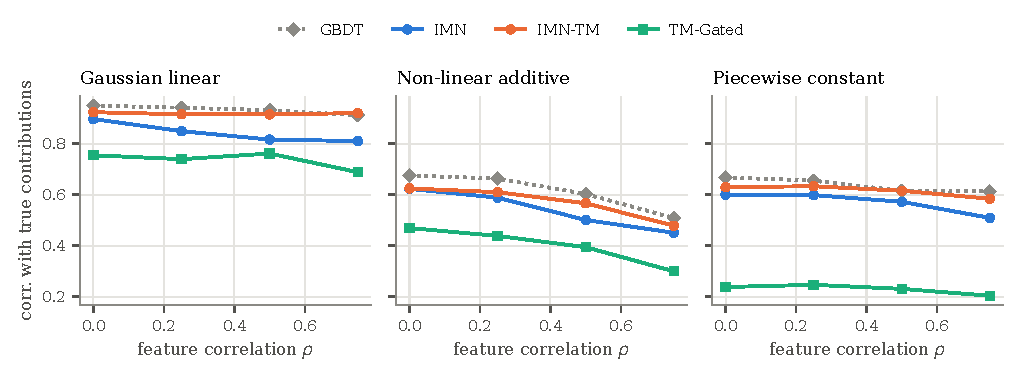
\includegraphics[width=\textwidth]{figures/xai_gt.pdf}
  \caption{\textbf{Attribution quality vs.\ feature correlation.} Mean over five seeds.}
  \label{fig:xai}
\end{figure}

\paragraph{IMN-TM explanations are closer to the truth than \imn{}'s.} Paired over the 60
tasks, the attributions of \arm{IMN-TM} correlate better with the true contributions than those
of \imn{} on \XaiVsimnWins{} of \XaiVsimnN{} tasks (mean \XaiVsimnMean, Wilcoxon
$p=\XaiVsimnP$).
\begin{itemize}
  \item \textbf{Piecewise constant.} The difference is clearest here: \Xaiimntmpiecewise{} for
        \arm{IMN-TM} vs.\ \Xaiimnpiecewise{} for \imn{}. In this family \imn{} is also less
        accurate (AUROC \XaiAucimnpiecewise{} vs.\ \XaiAucimntmpiecewise).
  \item \textbf{Gaussian linear.} Surprisingly, the difference also holds on the linear family
        (\Xaiimntmlinear{} vs.\ \Xaiimnlinear). As $\rho$ rises from 0 to 0.75, \imn{}'s
        correlation drops by \XaiLinDropimn{} and \arm{IMN-TM}'s by only \XaiLinDropimntm.
        With correlated inputs, a per-example hyperplane can shift weight between correlated
        features without changing its output. The TM-initialised clause weights are anchored
        to a global rule set and drift less.
\end{itemize}

\paragraph{Baselines.} The best global models remain ahead.
\begin{itemize}
  \item Plain logistic regression is nearly perfect on its own family (\Xailrlinear).
  \item GBDT's removal attributions beat \arm{IMN-TM} on \XaiVsgbdtLosses{} of the
        \XaiVsgbdtN{} tasks (\XaiVsgbdtMean, $p=\XaiVsgbdtP$).
\end{itemize}
The mesomorphic models are thus not more faithful than a removal-attributed tree ensemble.
Their advantage is that the explanation is the model's own local function, not a post-hoc
probe.

\paragraph{TM-Gated explanations are unreliable.} \arm{TM-Gated} is the least faithful method
in every family (\Xaitmgatedpiecewise{} on piecewise data; \arm{IMN-TM} is ahead on
\XaiVstmgatedWins/\XaiVstmgatedN{} tasks). Its local hyperplane is re-composed from rule-gated
pieces, and the removal of one feature switches rules on or off. The same failure appeared as
low local fidelity on real data (\S\ref{sec:interp}).
\subsection{Ablations}\label{sec:abl}
Each variant of Table~\ref{tab:abl} is run on the twelve Tier-1 datasets with seeds 0--2. It is
compared with the main-stage record of its reference arm on the same seeds, using a paired
Wilcoxon test over datasets without multiplicity correction. No variant changes test AUROC
significantly. Read together, the rows answer four design questions.

\paragraph{Basis size.} The source TM gains from more clauses (800 per class:
\AblTmEightMean, \AblTmEightWins/\AblTmEightLosses{} wins/losses, $p=\AblTmEightP$). IMN-TM
does not (\AblImntmEightMean, $p=\AblImntmEightP$), and 50 clauses per class are also enough
(\AblImntmFiftyMean, $p=\AblImntmFiftyP$). Re-weighting the clauses per example therefore
recovers what a larger TM gets by adding clauses, and the default of 200 is not a binding choice.

\paragraph{Initialisation.} Starting the generated weights at zero instead of at the TM's own
votes leaves accuracy unchanged (\AblNoinitMean, $p=\AblNoinitP$). It does lower local fidelity
from \AblNoinitRefFid{} to \AblNoinitFid. The initialisation is therefore an interpretability
device: it keeps the per-example weights close to a global rule set.

\paragraph{Generator input.} Feeding the clause outputs to the hypernetwork as well,
$[x, c(x)]$, is the worst variant (\AblXcMean, \AblXcWins/\AblXcLosses, $p=\AblXcP$). The
generator then sees the same binary evidence it is weighting, which appears to encourage
over-fitting. The raw input $x$ alone is the better choice.

\paragraph{Which clauses.} Random conjunctions matched to the trained clauses' firing rates give
nearly the same accuracy (\AblRandfrMean, $p=\AblRandfrP$), confirming the main-stage
random-clause control. Their local fidelity, however, drops from \AblRandfrRefFid{} to
\AblRandfrFid. The trained TM is not needed for accuracy, but it is what makes the explanations
generalise to the neighbourhood of an example.

\paragraph{Hybrid split.} Giving the linear block of IMN-Hybrid its own, weaker L1 penalty
($\lambda=0.1$) does not change accuracy (\AblSplitMean, $p=\AblSplitP$). The main-stage
hypothesis that the strong prior penalty suppressed a useful linear term is not supported.

\begin{table}[h]\centering\small
\caption{Ablations (Tier 1, seeds 0--2). $\Delta$ is the test AUROC change versus the reference
arm on the same seeds; $p$ is an uncorrected two-sided Wilcoxon test over datasets. The last
column is local fidelity at $k=10$.}\label{tab:abl}
\begin{tabular}{llcrcccc}
\toprule
Variant & reference & $n$ & mean $\Delta$ & W/L & $p$ & $\Delta$ vs.\ IMN & fid.\ $k{=}10$ \\
\midrule
TM, 50 clauses/class & TM & 12 & -0.0034 & 7/5 & 0.733 & -- & -- \\
TM, 800 clauses/class & TM & 12 & +0.0036 & 9/3 & 0.077 & -- & -- \\
IMN-TM on 50-clause TM & IMN-TM & 12 & +0.0004 & 6/6 & 0.850 & -0.0006 & 0.708 \\
IMN-TM on 800-clause TM & IMN-TM & 12 & -0.0012 & 8/4 & 0.622 & -0.0021 & 0.741 \\
IMN-TM without TM initialisation & IMN-TM & 12 & +0.0002 & 6/6 & 0.970 & -0.0007 & 0.649 \\
IMN-TM, generator input $[x, c(x)]$ & IMN-TM & 12 & -0.0116 & 5/7 & 0.064 & -0.0126 & 0.706 \\
IMN-TM, random clauses (rate-matched) & IMN-TM & 12 & -0.0017 & 8/4 & 0.850 & -0.0026 & 0.557 \\
IMN-Hybrid, linear $\lambda=0.1$ & IMN-Hybrid & 12 & +0.0003 & 8/4 & 0.339 & +0.0001 & 0.738 \\
\bottomrule
\end{tabular}
\end{table}
